% Standalone block diagrams of the four models compared in E1.
% Compile with pdflatex to produce fig_models_e1.pdf, then include it in the paper.
\documentclass[border=3pt]{standalone}
\usepackage{amsmath}
\usepackage{times}
\usepackage{tikz}
\usetikzlibrary{positioning,arrows.meta,calc,fit,backgrounds}
\begin{document}
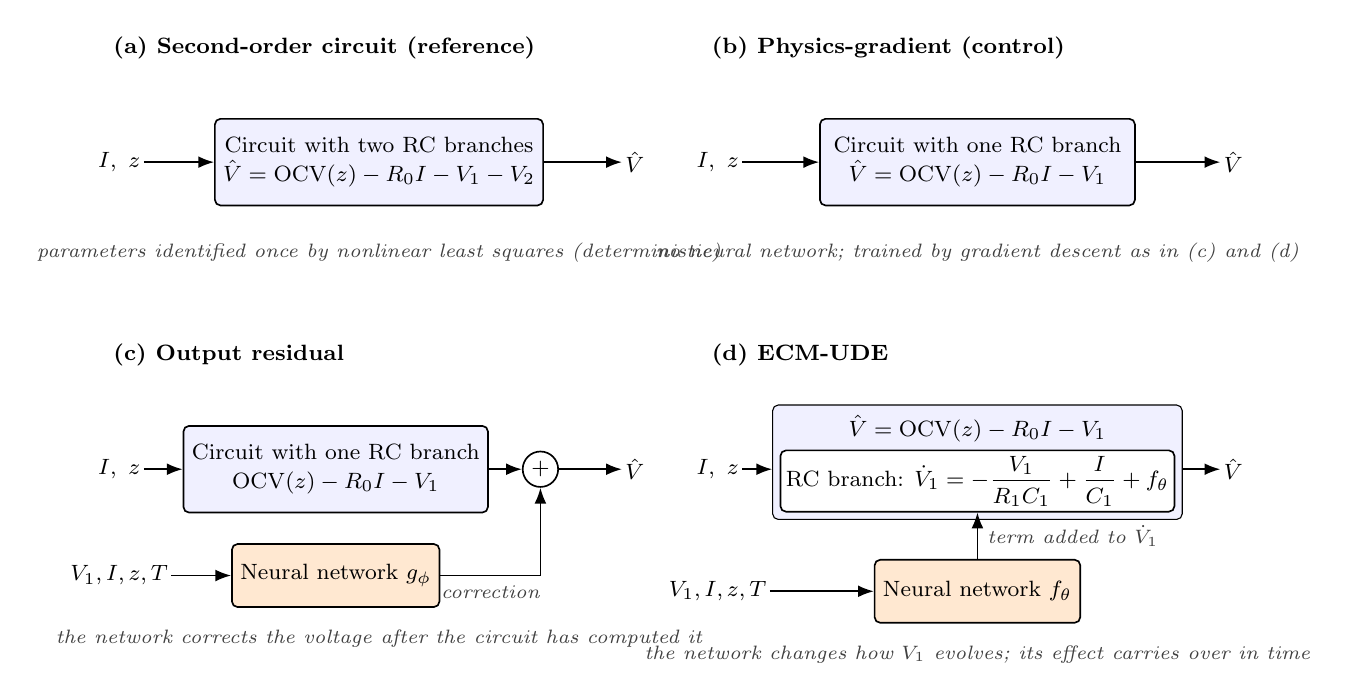
\begin{tikzpicture}[
  font=\footnotesize,
  >={Latex[length=2mm]},
  line width=0.6pt,
  inp/.style={align=center, inner sep=1pt},
  circ/.style={draw, rounded corners=2pt, fill=blue!6, align=center, minimum height=11mm, inner sep=3pt},
  state/.style={draw, rounded corners=2pt, fill=white, align=center, inner sep=2pt},
  nn/.style={draw, rounded corners=2pt, fill=orange!18, align=center, minimum height=8mm, inner sep=3pt},
  sum/.style={draw, circle, inner sep=0pt, minimum size=4.5mm, fill=white},
  tag/.style={font=\scriptsize\itshape, align=center, text=black!75},
  ttl/.style={font=\footnotesize\bfseries, anchor=west}
]

% ---------------- (a) reference: second-order circuit, NLS -----------------
\begin{scope}[shift={(0,0)}]
  \node[ttl] at (-0.2,2.05) {(a) Second-order circuit (reference)};
  \node[inp] (ia) at (0,0.6) {$I,\ z$};
  \node[circ, minimum width=40mm] (ca) at (3.3,0.6) {Circuit with two RC branches\\[1pt] $\hat V=\mathrm{OCV}(z)-R_0I-V_1-V_2$};
  \node[inp] (va) at (6.55,0.6) {$\hat V$};
  \draw[->] (ia) -- (ca); \draw[->] (ca) -- (va);
  \node[tag] at (3.3,-0.55) {parameters identified once by nonlinear least squares (deterministic)};
\end{scope}

% ---------------- (b) physics-gradient: first-order circuit, gradient -------
\begin{scope}[shift={(7.6,0)}]
  \node[ttl] at (-0.2,2.05) {(b) Physics-gradient (control)};
  \node[inp] (ib) at (0,0.6) {$I,\ z$};
  \node[circ, minimum width=40mm] (cb) at (3.3,0.6) {Circuit with one RC branch\\[1pt] $\hat V=\mathrm{OCV}(z)-R_0I-V_1$};
  \node[inp] (vb) at (6.55,0.6) {$\hat V$};
  \draw[->] (ib) -- (cb); \draw[->] (cb) -- (vb);
  \node[tag] at (3.3,-0.55) {no neural network; trained by gradient descent as in (c) and (d)};
\end{scope}

% ---------------- (c) output residual: network corrects the output ---------
\begin{scope}[shift={(0,-3.9)}]
  \node[ttl] at (-0.2,2.05) {(c) Output residual};
  \node[inp] (ic) at (0,0.6) {$I,\ z$};
  \node[circ, minimum width=34mm] (cc) at (2.75,0.6) {Circuit with one RC branch\\[1pt] $\mathrm{OCV}(z)-R_0I-V_1$};
  \node[sum] (sc) at (5.35,0.6) {$+$};
  \node[inp] (vc) at (6.55,0.6) {$\hat V$};
  \node[nn] (nc) at (2.75,-0.75) {Neural network $g_\phi$};
  \node[inp] (ic2) at (0,-0.75) {$V_1,I,z,T$};
  \draw[->] (ic) -- (cc); \draw[->] (cc) -- (sc); \draw[->] (sc) -- (vc);
  \draw[->] (ic2) -- (nc);
  \draw[->] (nc) -| node[pos=0.25, below, tag] {correction} (sc);
  \node[tag] at (3.3,-1.55) {the network corrects the voltage after the circuit has computed it};
\end{scope}

% ---------------- (d) ECM-UDE: network inside the RC dynamics --------------
\begin{scope}[shift={(7.6,-3.9)}]
  \node[ttl] at (-0.2,2.05) {(d) ECM-UDE};
  \node[inp] (id) at (0,0.6) {$I,\ z$};
  \node[state] (sd) at (3.3,0.45) {RC branch: $\dot V_1=-\dfrac{V_1}{R_1C_1}+\dfrac{I}{C_1}+f_\theta$};
  \node[inp, above=0.5mm of sd] (od) {$\hat V=\mathrm{OCV}(z)-R_0I-V_1$};
  \begin{scope}[on background layer]
    \node[circ, fit=(sd)(od), inner sep=2.5pt] (cd) {};
  \end{scope}
  \node[inp] (vd) at (6.55,0.6) {$\hat V$};
  \node[nn] (nd) at (3.3,-0.95) {Neural network $f_\theta$};
  \node[inp] (id2) at (0,-0.95) {$V_1,I,z,T$};
  \draw[->] (id) -- (cd.west|-id); \draw[->] (cd.east|-vd) -- (vd);
  \draw[->] (id2) -- (nd);
  \draw[->] (nd) -- node[right, tag] {term added to $\dot V_1$} (sd.south);
  \node[tag] at (3.3,-1.75) {the network changes how $V_1$ evolves; its effect carries over in time};
\end{scope}

\end{tikzpicture}
\end{document}
